\chapter{Convergence Diagnostics for the Long-Run Reference Reconstruction}
\label{app:baseline_convergence}

The \gls{nrmse} comparisons in Chapter~\ref{chapter:optimisation} use the final iterate of one long-run reconstruction as their reference image. This one-bed phantom reconstruction used the same objective as the 20-pass comparisons, but was continued for 1000 epochs with 36 stochastic updates per epoch, a Gershgorin-diagonal \gls{mm} preconditioner, and a more conservative relaxation rate of $\eta_{\mathrm{relax}}=10^{-4}$. Only one such reference run was performed.

Let $\mathcal O_k=\mathcal O(\bm z^{(k)})$ be the recorded objective after epoch $k$, and define
\begin{equation}
    \mathcal O^\star=\min_{0\leq k\leq 1000}\mathcal O_k.
    \label{eq:app_baseline_best_objective}
\end{equation}
Here $\mathcal O^\star$ is the best objective observed during this run. It is not a proven global minimum, and the reference image should likewise be understood as a long-run numerical reference rather than ground truth.

\begin{figure}[htbp]
    \centering
    \begin{subfigure}{0.49\linewidth}
        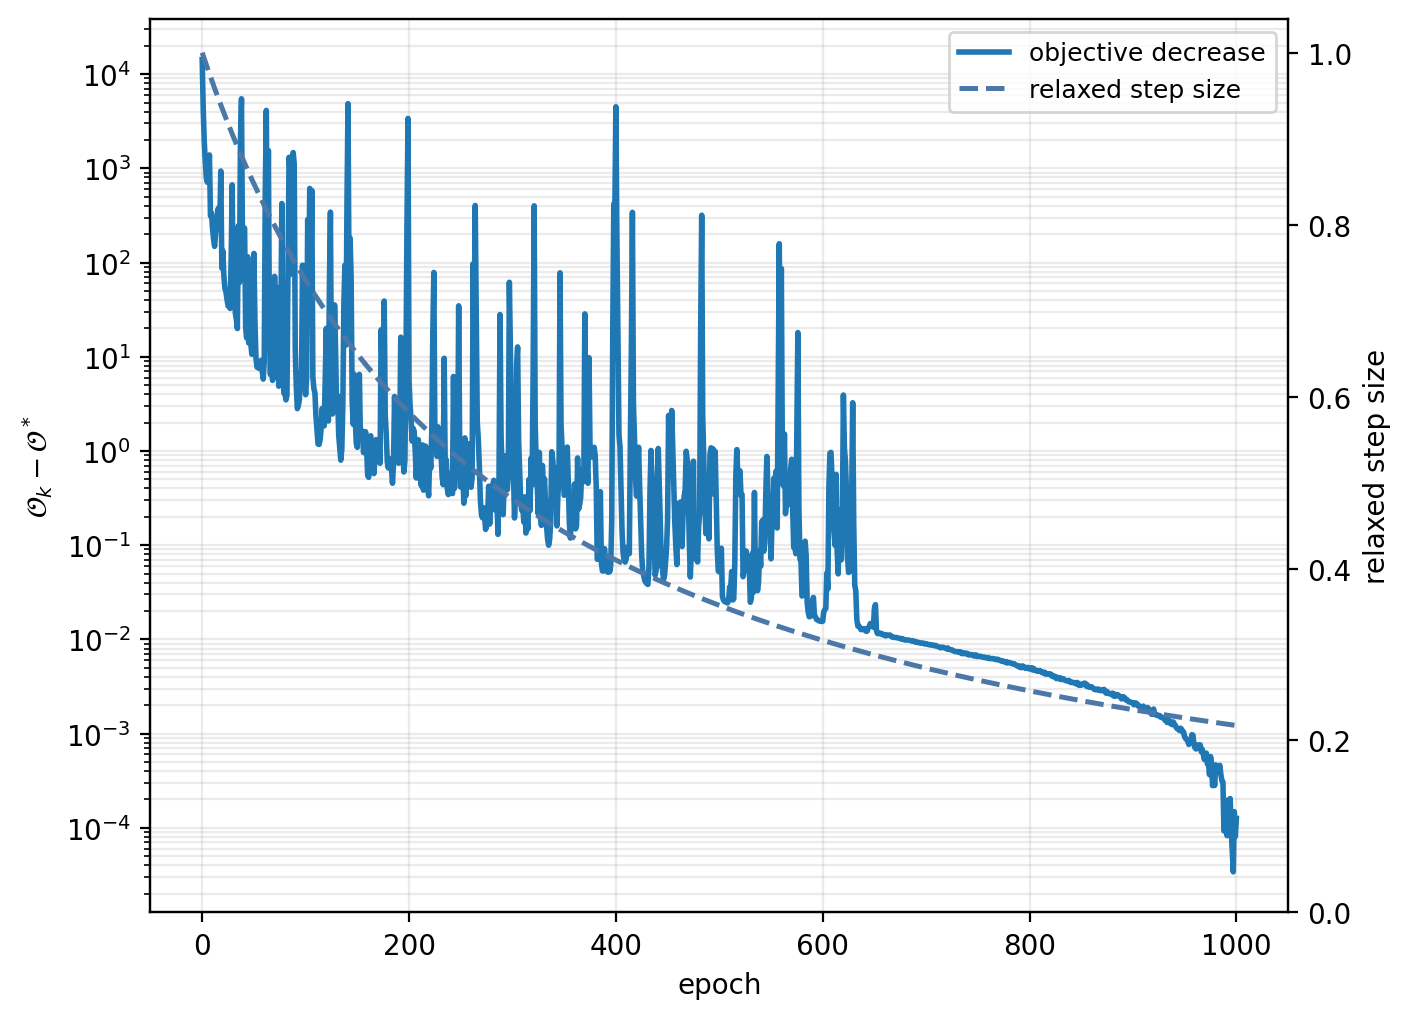
\includegraphics[width=\linewidth]{figures/preconditioning/baseline/baseline_convergence_final_objective_panel.png}
        \caption{Objective gap on a logarithmic scale.}
    \end{subfigure}
    \hfill
    \begin{subfigure}{0.49\linewidth}
        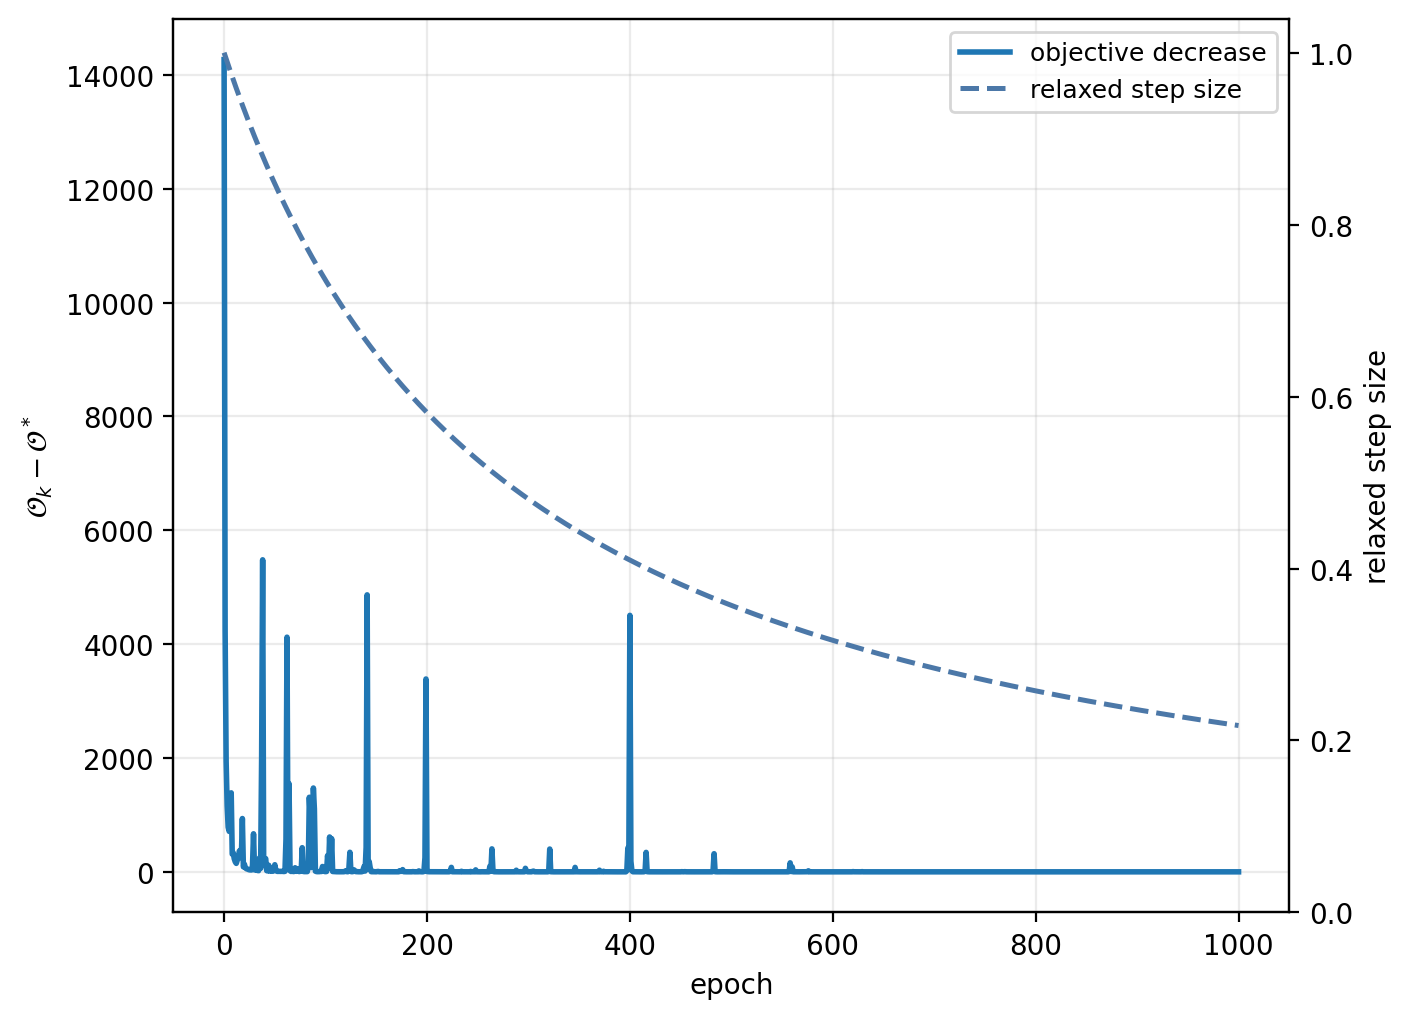
\includegraphics[width=\linewidth]{figures/preconditioning/baseline/baseline_convergence_final_objective_panel_linear.png}
        \caption{Objective gap on a linear scale.}
    \end{subfigure}
    \caption{Long-run objective diagnostics. The solid curve is $\mathcal O_k-\mathcal O^\star$ and the dashed curve is the relaxed step size. The linear view shows that most of the observed objective decrease occurs early, while the logarithmic view resolves the residual decrease over the complete 1000-epoch run.}
    \label{fig:app_baseline_objective}
\end{figure}

The objective contains stochastic excursions early in the run, but its gap relative to the best observed value becomes negligible. Table~\ref{tab:app_baseline_stationarity} reports the final objective and iterate diagnostics. The run had achieved 99.9\% of its total observed objective decrease by epoch 45, when the relaxed step remained $0.8606$.

\begin{table}[htbp]
    \centering
    \caption{Stationarity diagnostics for the 1000-epoch reference reconstruction.}
    \label{tab:app_baseline_stationarity}
    \small
    \begin{tabular}{p{0.68\linewidth}r}
        \toprule
        Quantity & Value\\
        \midrule
        Final objective gap / observed objective decrease & $8.819\times10^{-9}$\\
        Final relative objective change per epoch & $1.717\times10^{-11}$\\
        Final PET iterate velocity per epoch & $7.285\times10^{-8}$\\
        Final relaxed step size & $0.2174$\\
        Epoch reaching 99.9\% of observed decrease & $45$\\
        Step size at that epoch & $0.8606$\\
        \bottomrule
    \end{tabular}
\end{table}

\begin{figure}[htbp]
    \centering
    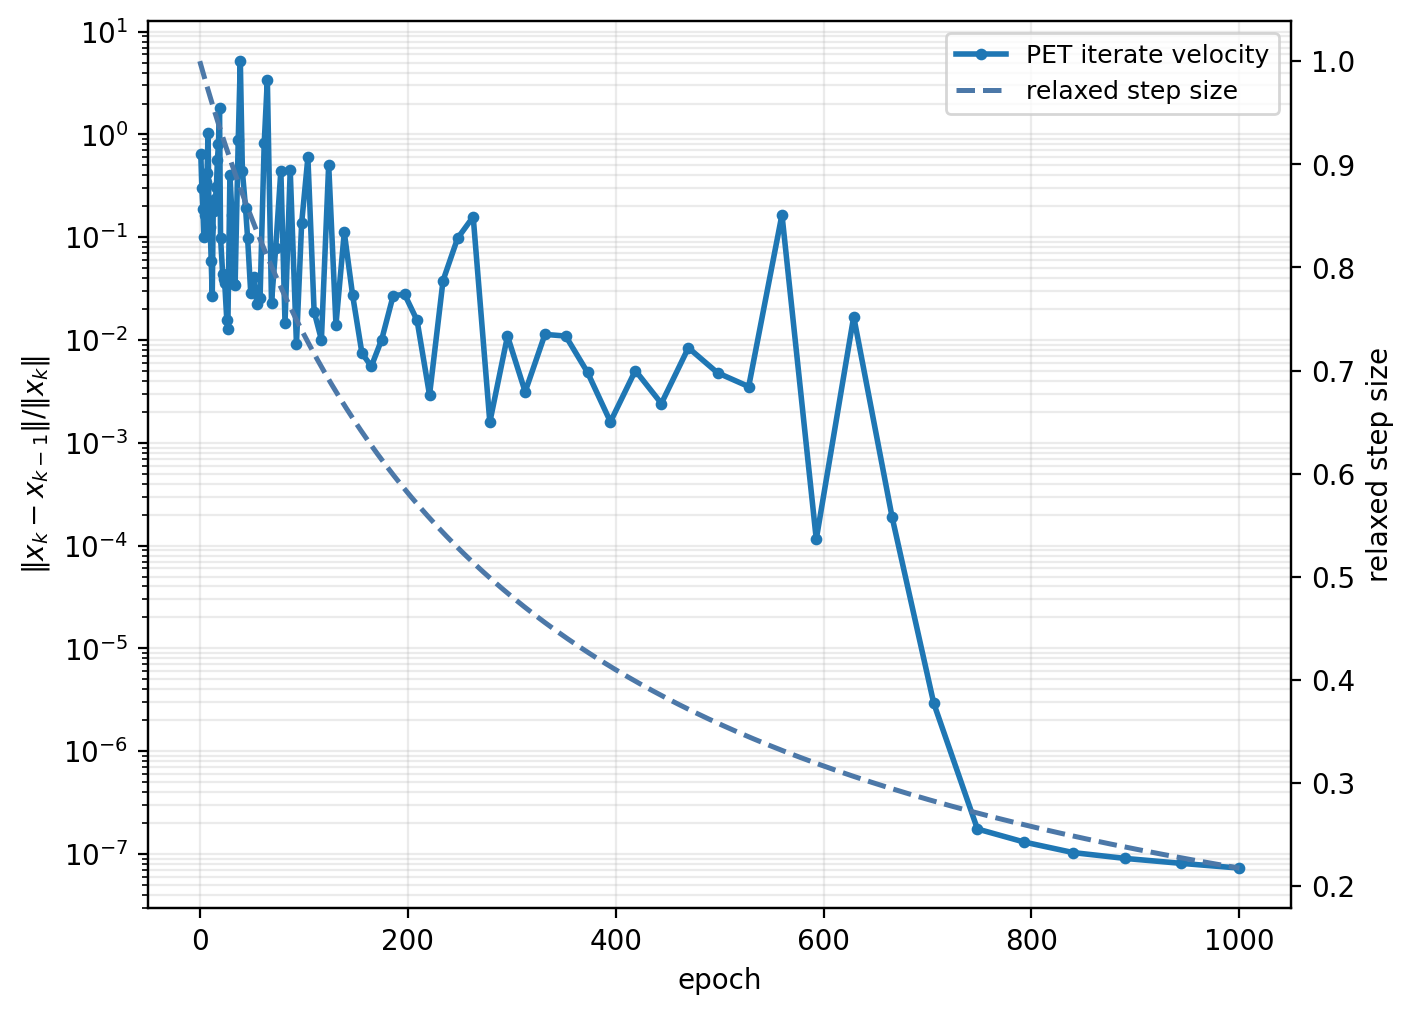
\includegraphics[width=0.82\linewidth]{figures/preconditioning/baseline/baseline_convergence_final_panel.png}
    \caption{Relative \gls{pet} iterate velocity, $\lVert x^{(k)}-x^{(k-1)}\rVert/\lVert x^{(k)}\rVert$, and relaxed step size during the long-run reference reconstruction. The final velocity is $7.285\times10^{-8}$ per epoch while the step size remains $0.2174$.}
    \label{fig:app_baseline_velocity}
\end{figure}

The final \gls{pet} and \gls{spect} iterates of this run are shown in Figure~\ref{fig:optim_reference_pair} of Chapter~\ref{chapter:optimisation}, alongside the regions over which the \gls{nrmse} curves are evaluated.

Together, the vanishing objective gap, relative objective change, and iterate velocity indicate that the reference was effectively stationary relative to the best observed iterate. The appreciable final step size makes step-size starvation an unlikely explanation for the plateau. These diagnostics support its use as a numerical reference for the short-run \gls{nrmse} comparisons, without asserting convergence to a global minimiser.
